\documentclass[xcolor={dvipsnames}]{beamer}

\usepackage[utf8]{inputenc}
\usepackage{amssymb, amsmath, amsthm, graphicx}

\usepackage{tikz}

\renewcommand{\phi}{\varphi}
\renewcommand{\epsilon}{\varepsilon}
\newcommand{\df}[1]{\textcolor{BrickRed}{\emph{#1}}}
\renewcommand{\th}[1]{\textcolor{Fuchsia}{\emph{#1}}}

\newcommand{\cX}{\mathcal{X}}
\newcommand{\cZ}{\mathcal{Z}}
\newcommand{\EE}{\mathbb{E}}

\DeclareMathOperator*{\argmin}{argmin}

\DeclareMathOperator{\Var}{Var}

\begin{document}

\begin{frame}
    \frametitle{Representation Learning}
\begin{quote}
    \normalfont \large
Learning representations of the data that make it easier to extract useful information when building classifiers or other predictors.

\bigskip
\begin{flushright}
\small \normalfont Y.\ Bengio, A.\ Courville, P.\ Vincent,\\ \emph{Representation Learning: A Review and New Perspectives},\\
    IEEE Transactions on Software Engineering, 2013.
\end{flushright}
\end{quote}
\end{frame}

\begin{frame}
    \frametitle{Data Transformation (Traditional)}
    \setlength{\parskip}{1em}

    Transform your data to facilitate model fitting, discrimination, etc.
    \begin{itemize}
        \setlength\itemsep{0.5em}
        \item $\log$-tranformation: $(x, y)\mapsto (\log x, y)$
        \item $\log$-$\log$-transformation: $(x, y)\mapsto (\log x, \log y)$
        \item Polynomial features: $(x,y)\mapsto \big((x,x^2,\ldots,x^n), y\big)$
        \item Basis functions: $(x,y)\mapsto \big(\big(b_1(x),b_2(x),\ldots,b_n(x)\big), y\big)$
    \end{itemize}

    Transformations choice informed by \df{domain knowledge}, \df{exploratory data analysis}, and \df{model selection criteria}.
    
    Not \df{learned from data}.
\end{frame}





\begin{frame}
    \frametitle{Supervised Representation Learning}
    \setlength{\parskip}{1em}

    \df{Hidden layers} in \df{deep, supervised models} do representation learning, feed learned representation to, e.g., a classifier.

    \begin{center}
        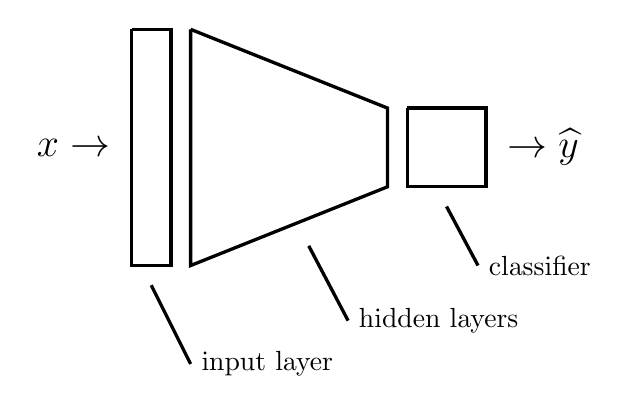
\begin{tikzpicture}
            \draw[very thick] (-3.0,1.5) -- (-0.5,0.5) -- (-0.5, -0.5) -- (-3.0, -1.5) -- (-3.0, 1.5);
            \draw[very thick] (-3.75, 1.5) -- (-3.25, 1.5) -- (-3.25, -1.5) -- (-3.75, -1.5) -- (-3.75, 1.5);

            \draw[very thick] (-0.25, 0.5) -- (0.75, 0.5) -- (0.75, -0.5) -- (-0.25, -0.5) -- (-0.25, 0.5);

            \node[right] at (0.9,0) {{\Large$\to\widehat{y}$}};
            \node[left] at (-3.9,0) {{\Large$x\to$}};


            \draw[very thick] (-3.5, -1.75) -- (-3.0, -2.75) node[right] {input layer};
            \draw[very thick] (-1.50, -1.25) -- (-1.00, -2.20) node[right] {hidden layers};
            \draw[very thick] (0.25, -0.75) -- (0.65, -1.5) node[right] {classifier};
        \end{tikzpicture}
    \end{center}
\end{frame}



\begin{frame}
    \frametitle{Transfer Learning}
    \setlength\parskip{1em}


    Typically, representations learned by hidden layers are sufficiently general to
    facilitate \df{transfer learning}, i.e., application to a different downstream
    task on a different --- often much smaller --- dataset.

    \df{Fine-tuning:} Training a \df{custom head} on the representation computed by a pretrained \df{base network}. 

    \begin{center}
        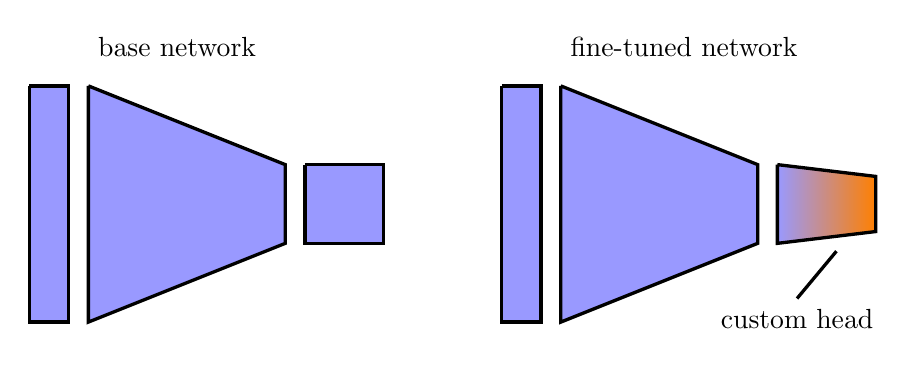
\begin{tikzpicture}
            \draw[very thick, fill=blue!40!white] (-3.0,1.5) -- (-0.5,0.5) -- (-0.5, -0.5) -- (-3.0, -1.5) -- (-3.0, 1.5);
            \draw[very thick, fill=blue!40!white] (-3.75, 1.5) -- (-3.25, 1.5) -- (-3.25, -1.5) -- (-3.75, -1.5) -- (-3.75, 1.5);

            \draw[very thick, fill=blue!40!white] (-0.25, 0.5) -- (0.75, 0.5) -- (0.75, -0.5) -- (-0.25, -0.5) -- (-0.25, 0.5);
            \node[right] at (-3.00,2.00) {base network};


            \begin{scope}[shift={(6,0)}]
                \draw[very thick, fill=blue!40!white] (-3.0,1.5) -- (-0.5,0.5) -- (-0.5, -0.5) -- (-3.0, -1.5) -- (-3.0, 1.5);
            \draw[very thick, fill=blue!40!white] (-3.75, 1.5) -- (-3.25, 1.5) -- (-3.25, -1.5) -- (-3.75, -1.5) -- (-3.75, 1.5);

            \shade[left color=blue!40!white, right color=orange, draw=black, very thick] (-0.25, 0.5) -- (1.00, 0.35) -- (1.00, -0.35) -- (-0.25, -0.5) -- (-0.25, 0.5);
            \node[right] at (-3.00,2.00) {fine-tuned network};

            \draw[very thick] (0.5, -0.6)-- (0,-1.20) node[below] {custom head};

              \end{scope}
        \end{tikzpicture}
    \end{center}
\end{frame}

\begin{frame}
    \frametitle{Self-Supervised Representation Learning}
    \setlength\parskip{1em}

    Learn useful representations of \df{unlabelled data} using a \df{pretext task} for which labels can be easily constructed.

    \begin{itemize}
        \setlength\itemsep{1em}
        \item Compression/Decompression (e.g., \df{autoencoders})
        \item Denoising (e.g., \df{denoising autoencoders})
        \item Image colorization
        \item Image inpainting
        \item Jigsaw puzzle solving
    \end{itemize}

    Use representation computed in solving pretext task for \df{downstream tasks}.
\end{frame}

\begin{frame}
    \frametitle{Autoencoders}
    \begin{itemize}
        \setlength\itemsep{1em}
    
        \item \df{data space}, $\cX$:  $\dim \cX\gg 0$
        
        \item \df{code space}, $\cZ$: $\dim \cZ \ll \dim \cX$
        
        \item \df{encoding map}, $E_\phi:$  $\cX\to\cZ$
        
        \item \df{decoding map}, $D_\theta:$  $\cZ\to\cX$
        
        \item \df{reconstruction:} $x \approx D_\theta(E_\phi(x)) =: \widehat{x}$
    \end{itemize}
    \end{frame}

\begin{frame}
    \frametitle{Autoencoders}

    \begin{center}
        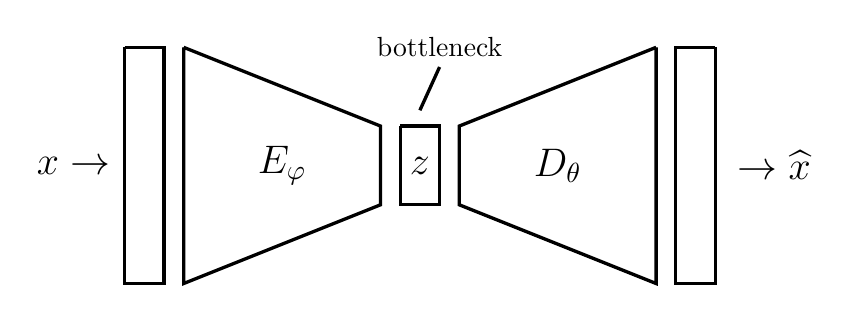
\begin{tikzpicture}
            \draw[very thick] (-3.0,1.5) -- (-0.5,0.5) -- (-0.5, -0.5) -- (-3.0, -1.5) -- (-3.0, 1.5);
            \draw[very thick] (-3.75, 1.5) -- (-3.25, 1.5) -- (-3.25, -1.5) -- (-3.75, -1.5) -- (-3.75, 1.5);
            \draw[very thick] (3.0,1.5) -- (0.5,0.5) -- (0.5, -0.5) -- (3.0, -1.5) -- (3.0, 1.5);
            \draw[very thick] (3.75, 1.5) -- (3.25, 1.5) -- (3.25, -1.5) -- (3.75, -1.5) -- (3.75, 1.5);

            \draw[very thick] (-0.25, 0.5) -- (0.25, 0.5) -- (0.25, -0.5) -- (-0.25, -0.5) -- (-0.25, 0.5);

            \draw[very thick] (0,0.7) -- (0.25, 1.25) node[above] {bottleneck};

            \node at (0,0) {{\Large$z$}};
            \node at (-4.4,0) {{\Large$x\to$}};
            \node at (-1.75,0) {{\Large$E_\varphi$}};
            \node at (4.5,0) {{\Large$\to\widehat x$}};
            \node at (1.75,0) {{\Large$D_\theta$}};
            \end{tikzpicture}
        \end{center}


    \begin{itemize}
        \setlength\itemsep{1em}

        \item $E_\phi$ and $D_\theta$ are typically neural networks.
        
        \item Weights $\phi$, $\theta$ are learned to minimize \df{reconstruction error}:
        \[
            (\phi^*,\theta^*) = \argmin_{(\phi, \theta)}\EE\left[\|\widehat x - x\|^2\right]
        \]

        \item \df{Bottleneck} forces the representation $z$ to retain only essential information about $x$.
    \end{itemize}
\end{frame}

\begin{frame}
    \frametitle{Application: Outlier Detection}
    \setlength\parskip{1em}
    If $x$ is an \df{outlier}, i.e., doesn't resemble an element of $\cX$, $\widehat x$ will likely be a poor reconstruction of $x$.

    Threshold reconstruction error to flag possible outliers.
    
    This is useful for detecting rare events, e.g., in fraud detection.

    Standard supervised learning techniques are difficult to apply to datasets with high
    \df{class imbalance}.

    What about \df{rare diseases}?
\end{frame}

\begin{frame}
    \frametitle{Autoencoders: Limitations}
    \setlength\parskip{1em}

    The representations learned by autoencoders aren't particularly useful for downstream tasks.

\begin{itemize}
    \setlength\itemsep{1em}
    \item To learn a useful representation, a pretext task has to be \df{semantically meaningful}.

    \item Pixel-by-pixel reconstruction loss doesn't encourage learning high level features of images.
    
    \item As $z'$ moves away from $z=E_\phi(x)$, $D_\theta(z')$ diverges visually from $D_\theta(z)$ very quickly.

\end{itemize}    

    \begin{center}
        \th{Euclidean distance $\neq$ perceptual distance}
    \end{center}

% Autoencoders don't capture enough global information about the distrubutions of $x$ and $z$ to allow for synthesizing data.
% \begin{itemize}
%     \setlength\itemsep{1em}
%     \item For randomly chosen $z\in\cZ$, $D_\theta(z)$ is unlikely to resemble an element of $\cX$.
%     % \item $E_\phi(\cX)$ is a ``thin'' subset of $\cZ$.
% \end{itemize}
\end{frame}

\begin{frame}
    \frametitle{Overcoming the Limitations}

    Decrease the local variability of $D_\theta$ by adding random noise to $x$:
    \[
        \widehat x = D_\theta(\underbrace{\overbrace{E_\phi(x)}^z + \epsilon}_{z'})
    \]
    The mapping $x\mapsto \widehat x$ is now \df{stochastic}.

    \begin{center}
        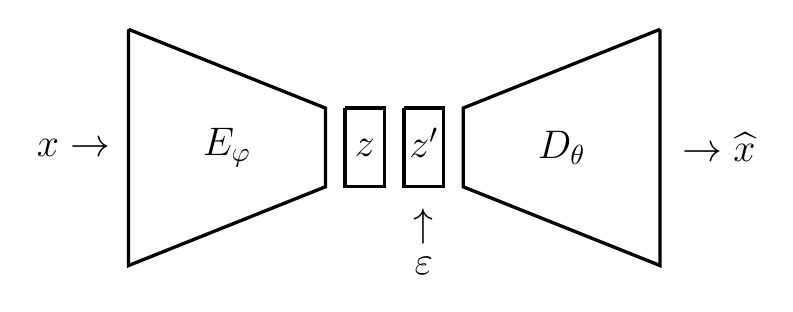
\begin{tikzpicture}
            \draw[very thick] (-3.0,1.5) -- (-0.5,0.5) -- (-0.5, -0.5) -- (-3.0, -1.5) -- (-3.0, 1.5);
            % \draw[very thick] (-3.75, 1.5) -- (-3.25, 1.5) -- (-3.25, -1.5) -- (-3.75, -1.5) -- (-3.75, 1.5);
            \draw[very thick] (3.75,1.5) -- (1.25,0.5) -- (1.25, -0.5) -- (3.75, -1.5) -- (3.75, 1.5);
            % \draw[very thick] (4.5, 1.5) -- (4, 1.5) -- (4, -1.5) -- (4.5, -1.5) -- (4.5, 1.5);

            \draw[very thick] (-0.25, 0.5) -- (0.25, 0.5) -- (0.25, -0.5) -- (-0.25, -0.5) -- (-0.25, 0.5);

            \draw[very thick] (0.5, 0.5) -- (1, 0.5) -- (1, -0.5) -- (0.5, -0.5) -- (0.5, 0.5);

            % \draw[very thick] (0,0.7) -- (0.25, 1.25) node[above] {bottleneck};

            \node at (0,0) {{\Large$z$}};
            \node at (0.75,0.06) {{\Large$z'$}};
            \node at (0.75,-1) {{\Large$\uparrow$}};
            \node at (0.75,-1.5) {{\Large$\epsilon$}};
            \node at (-3.7,0) {{\Large$x\to$}};
            \node at (-1.75,0) {{\Large$E_\varphi$}};
            \node at (4.5,0) {{\Large$\to\widehat x$}};
            \node at (2.5,0) {{\Large$D_\theta$}};
            \end{tikzpicture}
        \end{center}
\end{frame}

\begin{frame}
    \[
        \epsilon \sim N(0, I)
    \]
    \begin{center}
        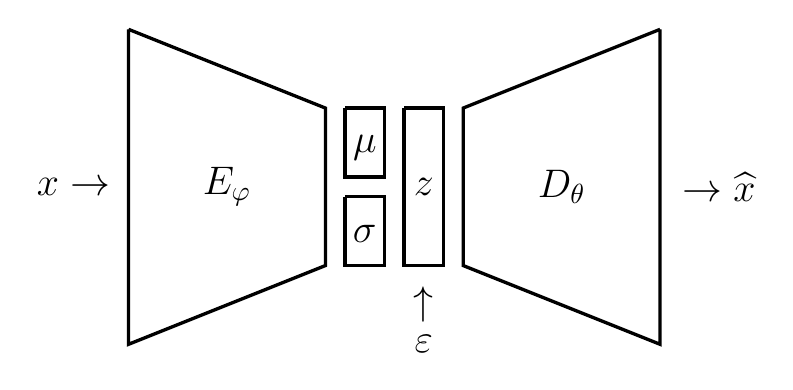
\begin{tikzpicture}
            \draw[very thick] (-3.0,2) -- (-0.5,1) -- (-0.5, -1) -- (-3.0, -2) -- (-3.0, 2);
            % \draw[very thick] (-3.75, 1.5) -- (-3.25, 1.5) -- (-3.25, -1.5) -- (-3.75, -1.5) -- (-3.75, 1.5);
            \draw[very thick] (3.75,2) -- (1.25,1) -- (1.25, -1) -- (3.75, -2) -- (3.75, 2);
            % \draw[very thick] (4.5, 1.5) -- (4, 1.5) -- (4, -1.5) -- (4.5, -1.5) -- (4.5, 1.5);

            \draw[very thick] (-0.25, 1) -- (0.25, 1) -- (0.25, 0.125) -- (-0.25, 0.125) -- (-0.25, 1);

            \draw[very thick] (-0.25, -0.125) -- (0.25, -0.125) -- (0.25, -1) -- (-0.25, -1) -- (-0.25, -0.125);

            \draw[very thick] (0.5, 1) -- (1, 1) -- (1, -1) -- (0.5, -1) -- (0.5, 1);
            % \draw[very thick] (0,0.7) -- (0.25, 1.25) node[above] {bottleneck};

            \node at (0,0.5) {{\Large$\mu$}};
            \node at (0,-0.6) {{\Large$\sigma$}};
            \node at (0.75,0.0) {{\Large$z$}};
            \node at (0.75,-1.5) {{\Large$\uparrow$}};
            \node at (0.75,-2) {{\Large$\epsilon$}};
            \node at (-3.7,0) {{\Large$x\to$}};
            \node at (-1.75,0) {{\Large$E_\varphi$}};
            \node at (4.5,0) {{\Large$\to\widehat x$}};
            \node at (2.5,0) {{\Large$D_\theta$}};
            \end{tikzpicture}
        \end{center}

        \[
            z|x = \mu + \sigma\odot\epsilon \sim N(\mu, \sigma\sigma^T)
        \]

% \[
%     (\phi,\theta) = \argmin_{(\phi,\theta)} \EE\left[\|x - \widehat x\|^2\right]
% \]
        % \medskip sThis is almost a variational autoencoder.    

\end{frame}
\begin{frame}
    \frametitle{Latent Variable Models}
    \setlength\parskip{1em}

    We want to view $\theta$ and $\phi$ as 

    Latent variable model:
    \begin{itemize}
        \setlength\itemsep{1em}
        \item $z\sim p(z),\quad x|z\sim p(x|z; \theta)$
        \item $z$ is a latent/hidden/explanatory variable; $x$ is observed
        % \item $\displaystyle p(x) = \int p(x|z;\theta)p(z)\,dz$
    \end{itemize}

    This is a \df{generative model}.
    To produce an element of $\cX$,
    \begin{itemize}
        \setlength\itemsep{1em}
        \item sample $z$ from $p(z)$,
        \item sample $x$ from $p(x|z;\theta)$.
    \end{itemize}
    Want: Estimates of $\theta$ and $p(z|x;\theta)$
\end{frame}


\begin{frame}
    \frametitle{Autoencoders and latent variable models}
    \setlength\parskip{1em}
    \begin{align*}
        \text{apply encoder $E_\phi$ to $x$}&\;\longleftrightarrow\;
        \text{sample from $p(z|x)$}\\[3ex]
        \text{apply dencoder $D_\theta$ to $z$}&\;\longleftrightarrow\;
        \text{sample from $p(x|z)$}
    \end{align*}


    % We want a encoder, $x\mapsto E_\phi(x)$, taking values in \df{Gaussian distributions on $\cZ$},
    % and a decoder, $z\mapsto D_\theta(z)$, taking values in $\cX$, such that
    % \begin{enumerate}
    %     \setlength\itemsep{1em}
    %     \item $z\sim N(0, I)$,
    %     \item $p(z|x)\approx E_\phi(x)$,
    %     % \item $p(x|z;\theta) = N(x|\theta(z))$,
    %     \item The \df{expected reconstruction error}, $\displaystyle\EE_{z\sim E_\phi(x)}\left[\|x - D_\theta(z)\|^2\right]$, is small.
    % \end{enumerate}

    % Assume:
    % \begin{itemize}
    %     \setlength\itemsep{1em}
    %     \item $p(z)\sim N(z|0,I)$
    %     \item $p(z|x)\approx  N(z|\mu(x|\phi), \sigma(x|\phi)^2)) =: q(z|x;\phi)$, so that
    %     \[
    %         E_\phi(x) = \big(\mu(x|\phi), \sigma(x|\phi)\big)
    %     \]
    %     \item $p(x|z) = N(x|\mu(z|\theta), \sigma^2)$ so that $E_\theta(z) = \mu(z|\theta)$
    % \end{itemize}
    
\end{frame}


\begin{frame}
    \frametitle{Variational Bayes}
    \setlength\parskip{1em}

    Set up an optimization problem to give us the maximum likelihood estimator of $\theta$.

    Maximize $\log$-likelihood, $p(x|\theta)$

    Bayes theorem gives:
    \[
        \log p(x) = \EE_{z\sim p(z|x)}\log p(x|z) - D[p(z|x)||p(z)]
    \]
    Approximate posterior $p(z|x)$ by $q(z|x)$:
    \[
        \log p(x) - D[q(z|x)||p(z|x)] = \EE_{z\sim q(z|x)}\log p(x|z) - D[q(z|x)||p(z)]
    \]
    Instead of maximizing $p(x)$, maximize the \df{lower bound}:
    \[
        \max_q\left(\EE_{z\sim q(z|x)}\log p(x|z) - D[q(z|x)||p(z)]\right)%\leq \log p(x)
    \]
    

\end{frame}

\begin{frame}
    \setlength\parskip{1em}

    \[
        \max_q\left(\EE_{z\sim q(z|x)}\log p(x|z) - D[q(z|x)||p(z)]\right)%\leq \log p(x)
    \]

    Use the Gaussian family for $q$:
    \[
    q(z|x;\phi) = N(z|\mu(x|\phi), \sigma(x|\phi)^2)) 
    \]

    Optimization problem becomes:
    \[
    \max_q\left(\EE_{\epsilon\sim N(0,I)}\log p(x|z=\mu(x) + \sigma(x)\odot\epsilon) - D[q(z|x)||p(z)]\right)%\leq \log p(x)
    \]

    This can be maximized by gradient descent.

    

\end{frame}

\end{document}